\documentclass{article}
\usepackage{cancel}
\usepackage[utf8]{inputenc}
\usepackage {titlesec}
\usepackage[english,russian]{babel}
\usepackage{graphicx}
\graphicspath{{pictures/}}
\usepackage{amsmath}
\titlespacing*{\section}{\parindent}{*4}{*4}
\begin{document}

\section{Задача 1}
	\textbf{а)} Поймем, что если две граф 2-раскрашиваемый, то никакие две вершины в раскраске соединенные ребром не окрашены в один цвет. Значит все вершины "главного" цикла покрашены через одну. Более формально: пронумеруем вершины от 0 до $ 2n - 1$, тогда вершины чей номер по модулю 2 равен 0, покрашены в первый цвет, а оставшиеся во второй цвет.
	Но вершина 0 и $n$ соединены ребром, как противоположные, а значит покрашены в разные цвета:
	\begin{center}
		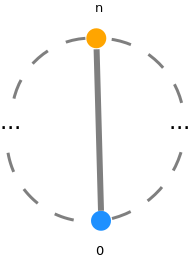
\includegraphics[scale=0.5]{1_1}
	\end{center}
	
	Но тогда $n$ и 0 имеют разную четность. Значит $n$ нечетно. Поймем, что такая раскраска правильная для всех нечетных $n$: любая вершина i, соединена с $ i + 1,\space i - 1,\space i + n + 1$ (по модулю 2n), четности которых отличаются, а значит различаются и цвета. $\Rightarrow$ граф 2-раскрашиваемый.
	
	\textbf{Ответ:} при нечетных $n$
	\\
	\textbf{б)} Очевидно, что раскраска из п. \textbf{а} для нечетных $n$ является также 3-х раскраской.
	Покажем, что 3-раскраска существует и для прочих $n$. Рассмотрим такую 3-раскраску:
	\begin{center}
	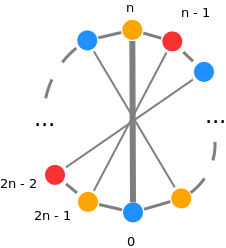
\includegraphics[scale=0.5]{1_2}
	\end{center}
	Вершины с 0 по $n - 2$, а также $2n - 1$ - четные номера 1ый цвет, нечетные - 2ой; Вершины с $n$ по $2n - 3$ - наоборот. Вершины $n - 1$ и $2n - 2$ покрасим цветом 3.
	Тогда все вершины с 0 по $n - 3$ будут соединены с вершинами, с $n$ по $2n - 3$, причем четность номеров совпадает, а цвет в зависимости от четности - инвертирован, значит цвета различны. А вершины $2n - 1$ и $n - 2$, $n$ и $2n - 1$ - содержат в себе по вершине третьего цвета, значит раскрашены правильно.
	
	Но данная раскраска не работает для $n = 2$. Но поймем, что при $n = 2$, наш граф полный на 4-х вершинах, а значит не 3-раскрашиваем (в чем можно убедиться перебором).
	
	\textbf{Ответ:} 3-раскраска для всех $n$, кроме 3.
\section{Задача 3}

Требуемый граф:
\\
\begin{center}
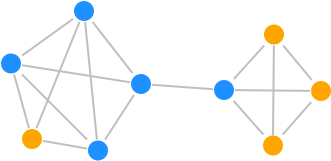
\includegraphics[scale=0.5]{3_1}
\end{center}

В нем есть мост, а значит нет Гамильтонова цикла: иначе можно взять вершину из левой компоненты пройтись по циклу и вернуться в нее, но тогда мы посетим правую компоненту, из которой можно вернуться только по мосту, по которому уже ходили.


\section{Задача 5}
\textbf{a)} Заметим, что в двудольном графе $K_{n,\space m}$ степень каждой вершины в доле с $n$ вершинами равна $m$, и наоборот: в доле с $m$ вершинами степень каждой равна $n$.
Но тогда для существования эйлерового цикла необходимо и достаточно, чтобы $\forall u \in V: d(u) = 2k$, значит эйлеров цикл существует, когда $n, \space m$ четны.

\textbf{Ответ:} при четных $n,\space m$.
\\
\textbf{б)} Допустим существование Гамильтонов цикла.

Раз граф двудольный, то он 2-раскрашиваемый, в нем более двух вершин и нет циклов нечетной длины $\Rightarrow$ Если в графе есть Гамильтонов цикл, то $n + m = 2k, \space k > 1$ как минимум. 
 
 Поймем, что если покрасить граф в два цвета, то любые две соседние вершины в цикле будут разных цветов. Значит если начать обход цикла, то после каждой пройденной вершины цвета $1$ будет идти вершина цвета $2$, т.к. вершины не повторяются и количество вершин четно, то каждой вершине цвета $1$ можно однозначно сопоставить вершину цвета $2$ (например следующую в порядке обхода цикла), а каждой вершине цвета $2$ можно однозначно сопоставить вершину цвета $1$ (предыдущую в порядке обхода). Но тогда число вершин цвета $1$ равно числу вершин цвета $2$. $\Rightarrow$ $$n = m$$
 
 Поймем, что двудольный граф, удовлетворяющий этому условию удовлетворяет и условию $n = m,\space n > 2$, то он является Гамильтонов графом. 
 В графе $K_{n,\space n}$ степень каждой вершины $n > |V| / 2$, а значит он удовлетворяет условию Дирака $\Rightarrow$ содержит цикл который мы от него хотим.

\textbf{в)} Если мы захотим, то убедимся, что этот явно полный двудольный граф $K_{6,6}$ - Эйлеров:

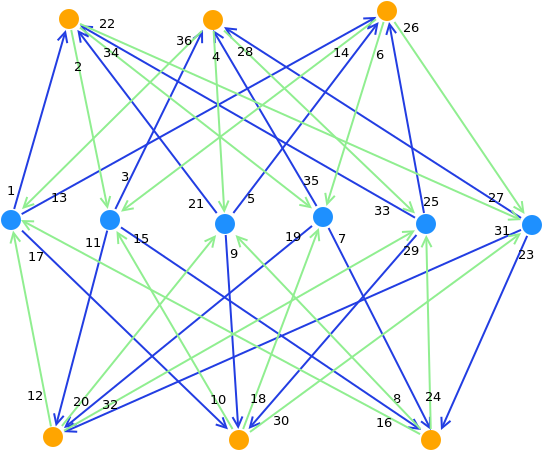
\includegraphics[scale=0.7]{5_1}
\newpage
А этот, Гамильтонов:

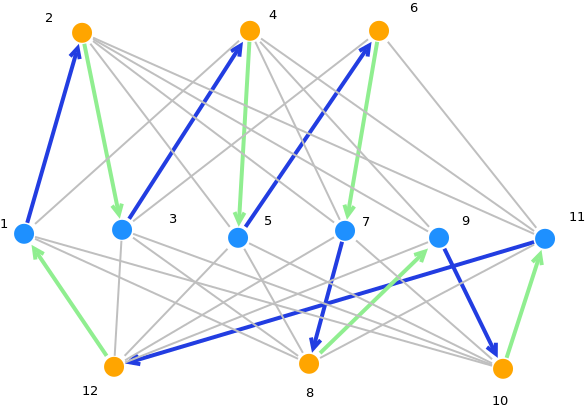
\includegraphics[scale=0.7]{5_2}

\section{Задача 6}

Разрешим в графах кратные ребра. Тогда определим маршрут, как последовательность ребер имеющих хотя бы один общий конец. Тогда путь - маршрут без повторяющихся ребер (ребра соединяющие одну и туже пару вершин будем считать различными). Тогда цикл - путь, в котором совпадает первая и последняя вершины. В частности цикл длины 2 может иметь такой вид:
\\
\begin{center}
	
\includegraphics[scale=0.6]{6_1}
\end{center}

Степень вершины по-прежнему: число ребер исходящих из нее.

Рассмотрим связный граф, в котором любые две вершины либо соединены 2-мя ребрами, либо не соединены вообще. Поймем, что в этом графе степень каждой вершины четна. Значит он граф Эйлера, т.е. по каждому можно пройти п всем ребрам по 1ому разу и вернуться в начало обхода.

Докажем признак графа Эйлера для связного графа(связный граф является графом Эйлера, когда все вершины имеют четную степень) с учетом разрешенных кратных ребер.

Выберем произвольную вершину графа $u_0$ и начнем строить из нее произвольный маршрут закрашивая ребра, по которым прошли цветом 1, и не двигаясь по уже закрашенным ребрам.
Заметим, что если мы попали в какую-либо вершину (не важно в какой раз) всегда сможем из нее выйти, т.к. ее степень четная, при этом мы закрасим два ее ребра, т.е. не изменим четность числа ребер, по которым можно попасть и покинуть эту вершину. С учетом того, что вершин конечное число,  на каком-то шаге мы вернемся в $u_0$. Если при этом все ребра графа уже закрашены, то получившийся маршрут и является Эйлеровым циклом (он не проходит ни по какому ребру дважды по построению и содержит все ребра). Иначе выбираем произвольную вершину $u_1$, принадлежащую закрашенному циклу из которой выходит хотя бы одно не закрашенное ребро. Повторяем с $u_1$  процедуру, произведенную с вершиной $u_1$, закрашивая ребра цветом 2.

Если еще не все ребра графа закрашены, то аналогичным образом выбираем вершину $u_2$ и т.д.

Так как число ребер графа конечно, то на каком-то шаге все ребра графа окажутся закрашенными. К этому моменту граф будет представлять собой объединение некоторого числа окрашенных разными цветами циклов, не имеющих общие ребра по построению.
Покажем методом математической индукции по числу полученных  циклов, что из них можно составить эйлеров цикл.

Базис индукции: два цикла.
Возьмем какую либо вершину $u$ из цикла цвета 1, пойдем по циклу, пока не найдем вершину $v$ принадлежащую циклу цвета 2. Пройдемся по нему, до возвращения в $v$ и завершим обход цикла цвета 1. Так как циклы не содержат общих ребер, то мы можем вернуться в $u$ пройдя все ребра циклов цвета 1 и 2 по одному разу $\Rightarrow$ получили цикл Эйлера. 

Педположение индукции.
Пусть после k описанных выше процедур все ребра графа окрашены.
Допустим, что  объединение k полученных  циклов, есть эйлеров цикл

Индуктивный переход.
Пусть после k+1 описанной выше процедуры все ребра графа окрашены. Докажем, что объединение k+1 полученного цикла, есть эйлеров цикл. Объединив любые k циклов в один, мы приходим к задаче объединения в эйлеров цикл двух циклов, которая описана в базе индукций.

Тогда поймем, что из способа пройтись по всем ребрам описанного в начале графа так, чтобы каждой было пройдено 
ровно 1 раз, вытекает способ пройтись по графу, без кратных ребер, посетив каждое ребро ровно два раза.

\textbf{Ответ:} Верно.

\section{Задача }

\end{document}